%%%%%%%%%%%%%%%%%%%%%%%%%%%%%%%%%%%%%%%%%
% Journal Article
% LaTeX Template
% Version 1.4 (15/5/16)
%
% This template has been downloaded from:
% http://www.LaTeXTemplates.com
%
% Original author:
% Frits Wenneker (http://www.howtotex.com) with extensive modifications by
% Vel (vel@LaTeXTemplates.com)
%
% License:
% CC BY-NC-SA 3.0 (http://creativecommons.org/licenses/by-nc-sa/3.0/)
%
%%%%%%%%%%%%%%%%%%%%%%%%%%%%%%%%%%%%%%%%%

%----------------------------------------------------------------------------------------
%	PACKAGES AND OTHER DOCUMENT CONFIGURATIONS
%----------------------------------------------------------------------------------------

\documentclass[twoside,twocolumn]{article}

\usepackage{blindtext} % Package to generate dummy text throughout this template 
\usepackage{verbatim}
\usepackage{listings}
\newcommand{\code}{\lstinline}
\usepackage[sc]{mathpazo} % Use the Palatino font
\usepackage[T1]{fontenc} % Use 8-bit encoding that has 256 glyphs
\linespread{1.05} % Line spacing - Palatino needs more space between lines
\usepackage{microtype} % Slightly tweak font spacing for aesthetics

\usepackage{amsmath, graphicx, graphics, float, amsfonts, xcolor, amssymb} % Image packages

\usepackage[english]{babel} % Language hyphenation and typographical rules

\usepackage[hmarginratio=1:1,top=32mm,columnsep=20pt]{geometry} % Document margins
\usepackage[hang, small,labelfont=bf,up,textfont=it,up]{caption} % Custom captions under/above floats in tables or figures
\usepackage{booktabs} % Horizontal rules in tables

\usepackage{lettrine} % The lettrine is the first enlarged letter at the beginning of the text

\usepackage{enumitem} % Customized lists
\setlist[itemize]{noitemsep} % Make itemize lists more compact

\usepackage{abstract} % Allows abstract customization
\renewcommand{\abstractnamefont}{\normalfont\bfseries} % Set the "Abstract" text to bold
\renewcommand{\abstracttextfont}{\normalfont\small\itshape} % Set the abstract itself to small italic text

\usepackage{titlesec} % Allows customization of titles
\renewcommand\thesection{\Roman{section}} % Roman numerals for the sections
\renewcommand\thesubsection{\roman{subsection}} % roman numerals for subsections
\titleformat{\section}[block]{\large\scshape\centering}{\thesection.}{1em}{} % Change the look of the section titles
\titleformat{\subsection}[block]{\large}{\thesubsection.}{1em}{} % Change the look of the section titles

\usepackage{fancyhdr} % Headers and footers
\pagestyle{fancy} % All pages have headers and footers
\fancyhead{} % Blank out the default header
\fancyfoot{} % Blank out the default footer
\fancyhead[C]{R lenguaje de programación $\bullet$ Jun 2022} % Custom header text
\fancyfoot[RO,LE]{\thepage} % Custom footer text

\usepackage{titling} % Customizing the title section

\usepackage{hyperref} % For hyperlinks in the PDF

%----------------------------------------------------------------------------------------
%	TITLE SECTION
%----------------------------------------------------------------------------------------

\setlength{\droptitle}{-4\baselineskip} % Move the title up

\pretitle{\begin{center}\Huge\bfseries} % Article title formatting
\posttitle{\end{center}} % Article title closing formatting
\title{Lenguaje R: una herramienta versátil para el análisis de datos} % Article title
\author{%
\textsc{Isaías Pérez Ramírez, Hugo Francisco Rincón López,} \\[1ex] % Your name
\textsc{Rudesindo Acuña Sánchez} \\[1ex] % Your name
\normalsize Universidad Nacional de Colombia - sede La Paz \\ % Your institution
\normalsize \href{mailto:isperezr@unal.edu.co}{isperezr@unal.edu.co,}
\normalsize \href{mailto:hufrinconlo@unal.edu.co}{hufrinconlo@unal.edu.co,}
\normalsize \href{mailto:ruacunas@unal.edu.co}{ruacunas@unal.edu.co}% Your email address
%\and % Uncomment if 2 authors are required, duplicate these 4 lines if more
%\textsc{Jane Smith}\thanks{Corresponding author} \\[1ex] % Second author's name
%\normalsize University of Utah \\ % Second author's institution
%\normalsize \href{mailto:jane@smith.com}{jane@smith.com} % Second author's email address
}
\date{\today} % Leave empty to omit a date
\renewcommand{\maketitlehookd}{%
\begin{abstract}
\noindent En 1970 los laboratorios Bell crearon un lenguaje de programación llamado S, que tenía como propósito brindar un enfoque alternativo y más interactivo en el campo de análisis de datos. Más adelante, dicho lenguaje derivó a lo que hoy se conoce como lenguaje de programación R. Este entorno de programación es una poderosa herramienta para análisis estadísticos y creación de gráficos. R tiene la ventaja de ser gratis, tener numerosos paquetes de mucha ayuda para multiples cálculos y tener en su página web muchas guías y ayudas para la correcta implementación de sus comandos. En el siguiente documento se abordarán aspectos generales para la instalación y el uso del lenguaje R. 


In 1970 Bell Labs created a programming language called S, which was intended to provide an alternative and more interactive approach to data analysis. This language later evolved into what is known today as the R programming language. This programming environment is a powerful tool for statistical analysis and graphing. R has the advantage of being free, having numerous packages of much help for multiple calculations and having in its web page many guides and aids for the correct implementation of its commands. The following document will address general aspects for the installation and use of the R language.


\end{abstract}
}

%----------------------------------------------------------------------------------------

\begin{document}

% Print the title
\maketitle

%----------------------------------------------------------------------------------------
%	ARTICLE CONTENTS
%----------------------------------------------------------------------------------------

\section{Instalación}

Antes de la instalación, es importante tener en cuenta que se debe descargar tanto R como Rstudio. Rstudio funciona como un IDE que brinda un entorno más agradable del lenguaje R. Si bien no es obligatorio descargar ambos programas, se recomienda hacerlo para facilitar la visualización de los datos.

\subsection{Instalación de R}
El primer paso para la instalación del lenguaje R consiste en ingresar a la página web de R (http://www.r-project.org/). A partir de ahí, se tienen en cuenta los siguientes pasos:
\begin{enumerate}
    \item click download CRAN in the left bar.
    \item choose a download site.
    \item choose Windows as target operation system.
    \item click base
    \item choose Download R 3.0.3 for Windows and
choose default answers for all questions
\end{enumerate}

% vspace (con espacio negativo)

\subsection{Instalación de Rstudio}
Al igual que la instalación del lenguaje R, para la descarga del Rstudio se realiza un protocolo semejante. El primer paso consiste en ingresar a la pagina web de Rstudio (http://www.rstudio.org/) y por último se efectúan los siguientes pasos. 
\begin{enumerate}
    \item click Download RStudio
    \item click Download RStudio Desktop
    \item click Recommended For Your System.
    \item  download the .exe file and run it (choose default
answers for all questions)
\end{enumerate}

De forma alternativa, Rstudio también cuenta con un servidor en línea que se puede usar en lugar de descargar el programa. Dicho programa recibe el nombre de Rstudio Cloud (https://rstudio.cloud/), y se puede usar de forma gratuita, aunque existe una versión paga con mejores características y más capacidad de almacenado. Para su ingreso, es necesario vincular una cuenta de usuario. 
%------------------------------------------------

\section{Estructuras de datos básicas de R}

Las estructura de datos se conocen como las formas de organización y manipulación de datos para posterior análisis y presentación. El lenguaje R maneja tres principales estructuras de datos: vectores, matrices y data frames. 

\subsection{Vectores}

Para definir un vector en lenguaje R es necesario hacer uso de la función c(). Si se desea crear un vector con los números del 1 al 10, el vector debe ser escrito de la siguiente forma:\\
\begin{verbatim}
x = c(1,2,3,4,5,6,7,8,9,19)
print(x)
\end{verbatim}

La primer línea de código indica que al vector lo hemos almacenado en una variable llamada x. Además, con la función \code{c()} creamos un vector que va de 1 a 10. Con la siguiente línea de código indicamos que imprima el vector en consola.  \newline
Es importante resaltar que dentro de un vector pueden estar números, valores logicos (booleanos), cadenas de caracteres y valores complejos. Incluso pueden estar diferentes tipos de datos dentro de un mismo vector. \break

En el caso de que se quiera generar un vector con valores aleatorios, hacemos uso de la función rnorm(). Dicha función hace parte del paquete que tiene R para estudiar distribuciones normales. Con rnorm() obtenemos valores aleatorios dentro una media y varianza establecidas.  La función se usa de la siguiente manera:\\
\begin{verbatim}
y = rnorm(100)
print(y)    
\end{verbatim}

\subsection{matrices}

La matrices en R son objetos donde los datos son almacenados en un conjunto rectangular bidimensional. La matrices son muy útiles para la organización y posterior análisis de datos. 

Para la creación de matrices en lenguaje R se usa la función:
\begin{verbatim}
    matrix(data, nrow, ncol, byrow=F)
\end{verbatim}
Donde el parametro "data" hace referencia a los valores estarán dentro de la matriz, "nrow" hace referencia al número de filas de la matriz, "ncol" es el número de columnas de la matriz y, por último, "byrow" sirve para indicar si los datos se colocan por filas o columnas. Como ejemplo de la función de matrix(data, nrow, ncol, byrow=F) tenemos el siguiente:

\begin{verbatim}
x <- matrix(c(2, 7, 1, 3, 6, 1), 
ncol = 2, byrow = TRUE)  
\end{verbatim}

Además de la función Matriz() existen otros comandos de mucha ayuda para el manejo de las matrices. Dichas funciones son: 

\begin {itemize}
\item dim(): Devuelve las dimesiones de la matriz.
\item dimnames(): Devuelve el nombre de las dimensiones de la matriz.
\item colnmaes(): Devuelven el nombre de las columnas de la matriz.
\item rownames(): Devuelve el nombre de las filas de la matriz.
\item length(): Devuelve la cantidad de elementos de la matriz.
\item apply(): Aplica una función sobre las filas o columnas de una matriz.
\item cbind(): Añade una columna a la matriz.
\item rbind(): Añade una fila a la matriz.
\end {itemize}

\subsection{Data frame}

Un dataframe es una estructura de datos similar a una matriz en la que las columnas son vectores y tienen un nombre, parecido a una tabla. Es muy utilizada para trabajar con cantidades de datos grandes. A diferencia de las matrices, un dataframe puede tener distintos tipos de datos en cada columna. Las operaciones ariméticas se vectorizan y aplican a todo el dataframe.

Para crear un dataframe se puede hacer de la siguiente manera:

\begin{verbatim}
    df <- data.frame(
    "entero" = 1:4, 
    "factor" = c("a", "b", "c", "d"), 
    "numero" = c(1.2, 3.4, 4.5, 5.6),
    "cadena" = as.character(c("a","b"))
    )
\end{verbatim} 

En este caso el comando \verb |data.frame| recibe el nombre de la columna entre comillas y un vector que ubica en dicha columna, estos vectores deben ser de igual tamaño.

Cuando se quiere acceder a una columna del dataframe se hace de la siguiente manera.

\begin{verbatim}
    df$col_name
\end{verbatim}

Usando el signo dólar y colocando el nombre de la columna. Este devuelve todos los datos de esta columna.

\section{Visualizaciones}

Al ser R un lenguaje de programación estadístico dispone de visualizaciones como histogramas, lineplots, barplots, boxplots, scatter plots, heatmaps, entre otras.

A continuación se enseñarán algunas gráficas muy usadas para exploración de datos. En las gráficas se usan hasta tres vectores data1, data2 y data3, conformados por 100 valores aleatorios cada uno.

Hay ciertos parámetros dentro de los gráficos que son comunes en los códigos, algunos de esos son:

\begin{enumerate}
    \item[main] Se utiliza para asignar un nombre al gráfico, este saldrá encima y en grande.
    \item[xlab] Se utiliza para asignar un nombre al eje x.
    \item[ylab] Se utiliza para asignar un nombre al eje y.
    \item[col] permite cambiar el color de los gráficos.
    \item[horiz] Este parámetro se utiliza en algunos casos para cambiar la orientación de algunos gráficos como los de barras o boxplots.
\end{enumerate}

\subsection{Gráfico de barras}

\begin{center}
    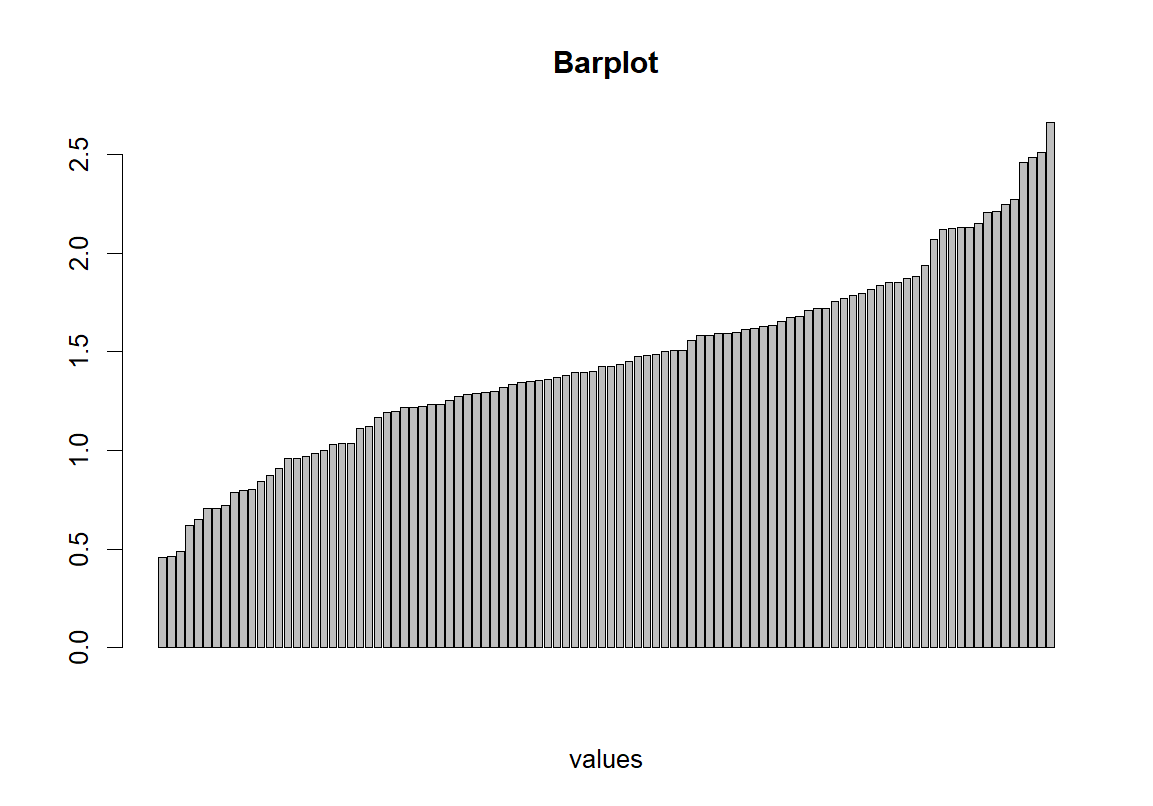
\includegraphics[width=0.4\textwidth]{images/barplot.png}
\end{center}

Estos son usados para analizar cambios en el tiempo de los datos y observar tendencias. Para crearlo se usando la función barplot().

\begin{verbatim}
    barplot(data1, main='Barplot', 
        xlab='values', col = 'gray', 
        horiz = F)
\end{verbatim}

\subsection{Histograma}

\begin{center}
    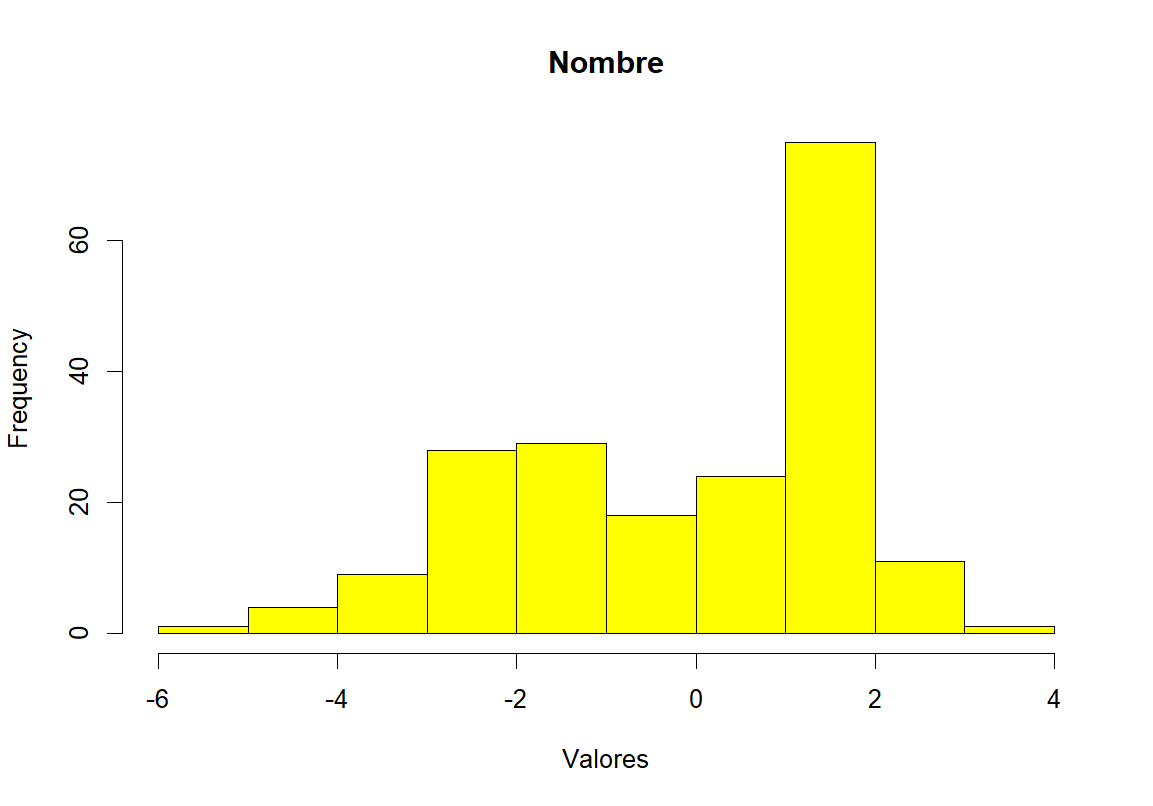
\includegraphics[width=0.4\textwidth]{images/hist.png}
\end{center}

Un histograma permite ver la frecuencia de los valores en ciertos rangos y se crea con la función hist()

\begin{verbatim}
    hist(c(data1,data2), 
     main ="Nombre", xlab ="Valores",
     col ="yellow",
     )
\end{verbatim}

\subsection{Gráfico de dispersión}

\begin{center}
    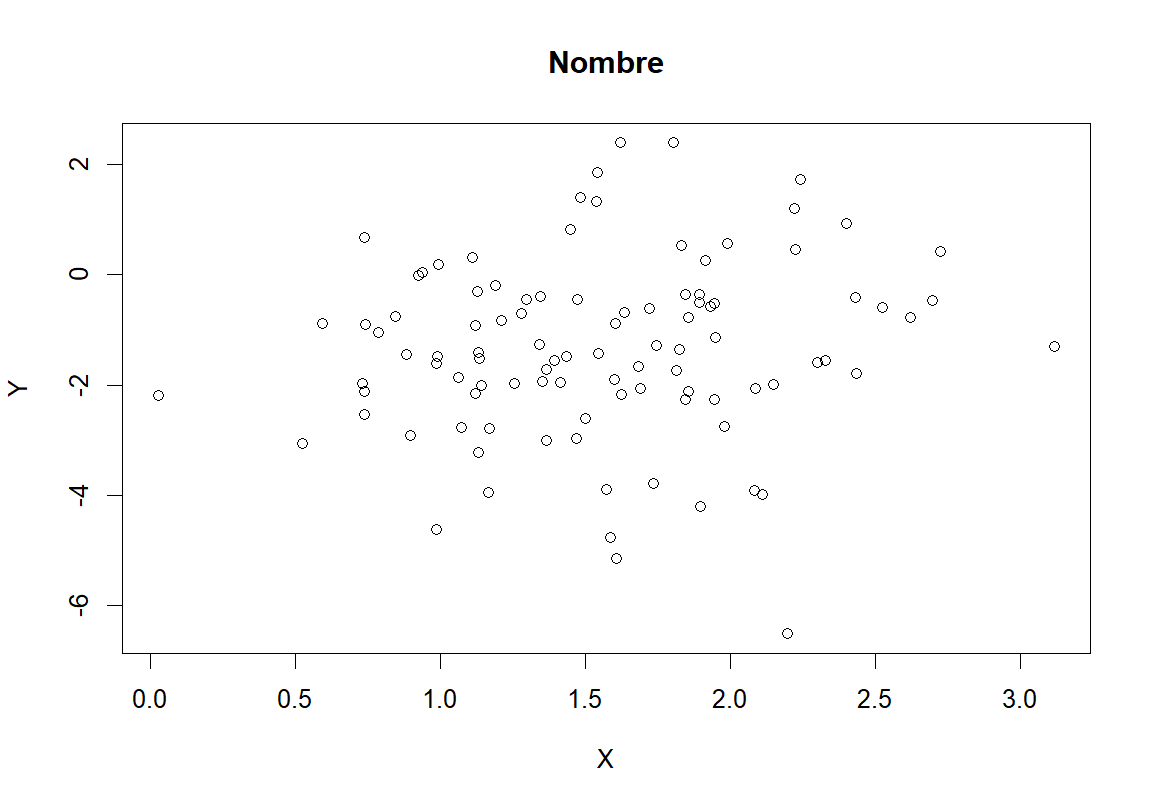
\includegraphics[width=0.4\textwidth]{images/scatter.png}
\end{center}

Esta visualización permite observar la dispersión de los datos, es útil para encontrar agrupaciones y patrones. Se crea usando el comando \verb|plot|

\begin{verbatim}
    plot(data1, data2, main ="Nombre",
     xlab = "X", ylab = "Y"
     )
\end{verbatim}

\subsection{Boxplot}

\begin{center}
    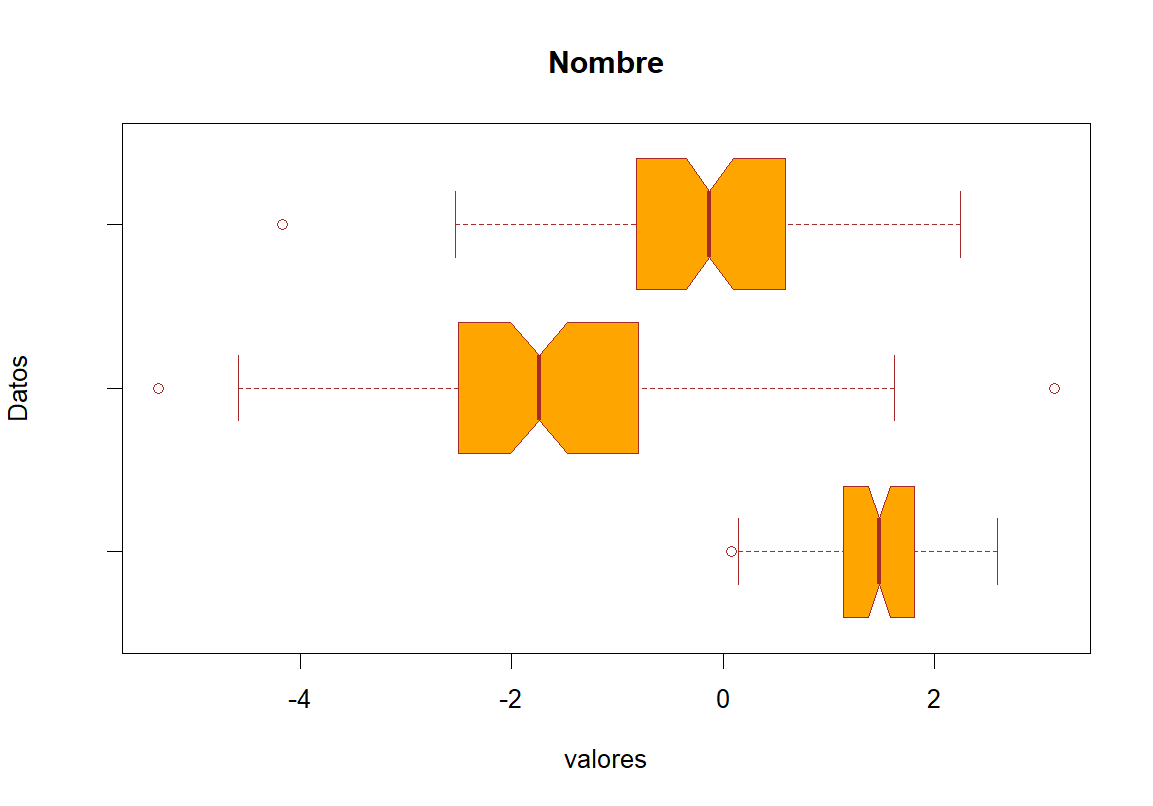
\includegraphics[width=0.4\textwidth]{images/boxplot.png}
\end{center}

En el boxplot se puede observar un resumen de los datos. El máximo, el mínimo, la mediana, cuartiles y valores atípicos de los datos. Para generar uno se utiliza el comando \verb|boxplot|

\begin{verbatim}
    boxplot(data1, data2, data3, 
        main = "Nombre",xlab="valores",
        ylab = "Datos", col = "orange",
        border = "brown",
        horizontal = T, notch = T)
\end{verbatim}

En este caso se puede observar que la gráfica está en modo horizontal, el comando \verb|notch| activa la forma diferente del gráfico y \verb|border| cambia el color de los marcos para hacerlos más notables.

\subsection{Mapa de calor}

\begin{center}
    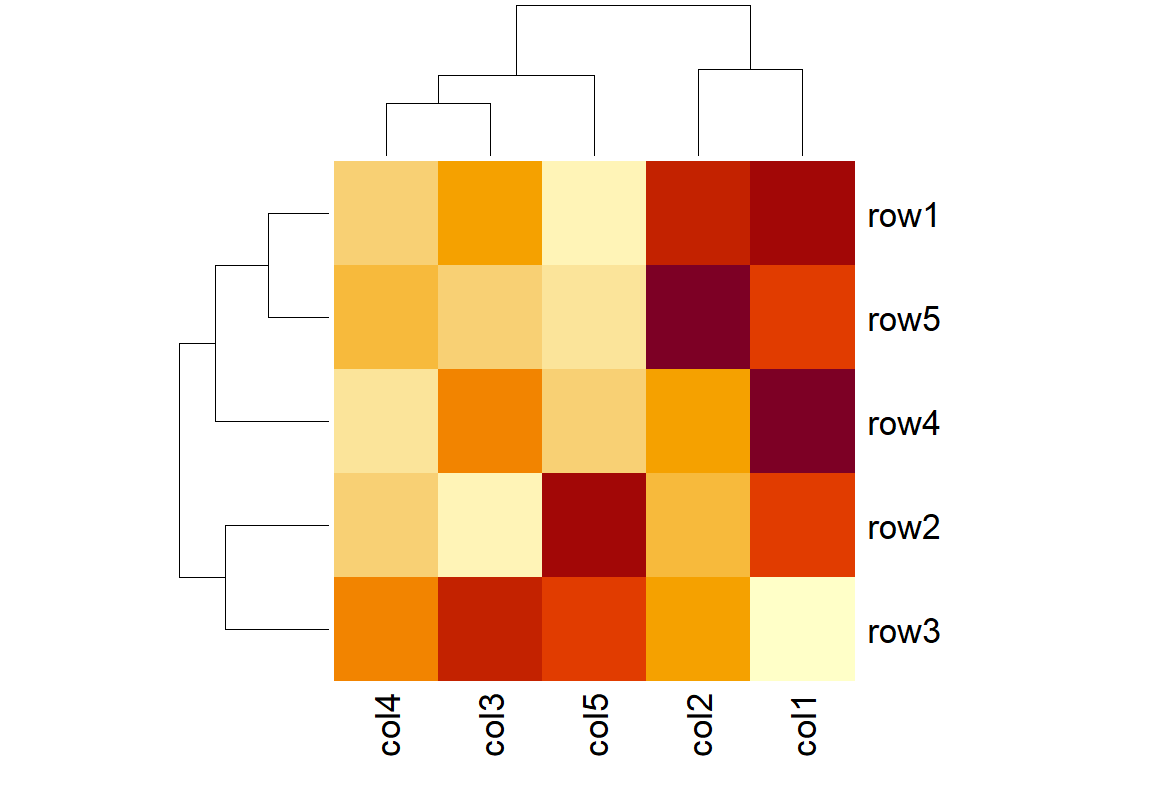
\includegraphics[width=0.4\textwidth]{images/heatmap.png}
\end{center}

Los mapas de calor sirven para ver diferentes valores en una tabla usando colores, son de gran utilidad para comparar matrices de correlación. Para generarla se usa el código \verb|heatmap|

\begin{verbatim}
    data <- matrix(rnorm(25, 0, 5),
        nrow = 5, ncol = 5)
    colnames(data) <-paste0("col", 1:5)
    rownames(data) <-paste0("row", 1:5)
    heatmap(data)   
\end{verbatim}

En este caso se utiliza una matriz 5x5 de valores aleatorios. Se le asignan nombres de col1 hasta col5 a las columnas y row1 hasta row5 a las filas. 


%----------------------------------------------------------------------------------------
%	REFERENCE LIST
%----------------------------------------------------------------------------------------

\begin{thebibliography}{99} % Bibliography - this is intentionally simple in this template

\bibitem[bhartirishika, 2022]{}\textit{Data Visualization in R}. Geeksforgeeks. https://www.geeksforgeeks.org/data-visualization-in-r/

\bibitem[RDocumentation]{}https://www.rdocumentation.org/

\bibitem[Figueredo and Wolf, 2009]{Figueredo:2009dg}
Figueredo, A.~J. and Wolf, P. S.~A. (2009).
\newblock Assortative pairing and life history strategy - a cross-cultural
  study.
\newblock {\em Human Nature}, 20:317--330.
 
\end{thebibliography}

%----------------------------------------------------------------------------------------

\end{document}


%R (vectores, matrices y data frames) y su manipulaci ́on.

%– Opciones y ejemplos de visualizaci ́on de datos.

%– Incluir la bibliograf ́ıa y citar las fuentes de donde se tom ́o la infr

%2. Dise ̃nar una versi ́on resumida del tutorial en formato de diapositivas o ṕoster.
%3. Compartir el documento y su c ́odigo fuente, y las diapositas o p ́oster v́ıa Github.